\chapter{関連研究}
\label{rw}

\begin{figure}[h]
	\begin{center}
		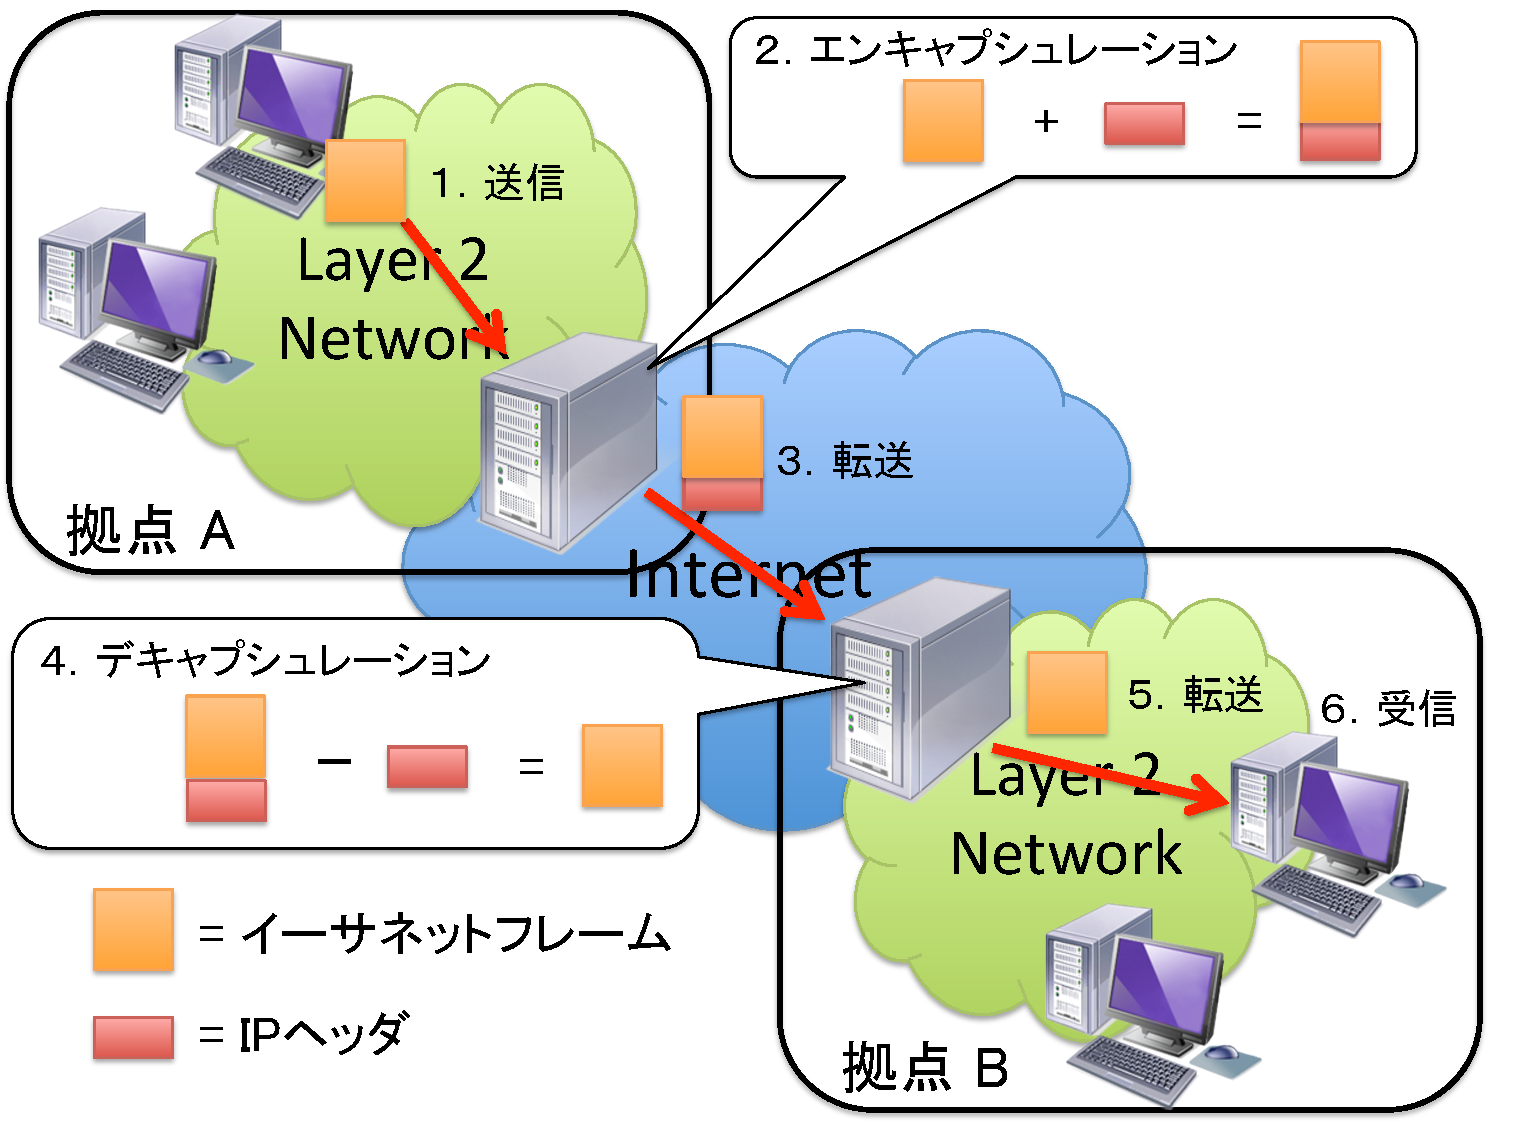
\includegraphics[scale=0.50]{./img/l2tunnel}
		\caption{Layer 2ネットワークの拡張手法}
		\label{img:l2tunnel}
	\end{center}
\end{figure}

Layer 2ネットワーク拡張技術を利用することにより、インターネット上に分散された複数の拠点に同一の
Layer 2ネットワークを拡張することができる。広域に分散した複数の拠点でサービスを展開するためには、
サービスを構成しているコンポーネントを拠点間で共有する必要がある場合が多い。広域に分散した複数の拠点間で
、共通のセキュリティーポリシーが適用された状態で、共通のコンポーネントを利用する手法の1つとしてLayer 2ネットワーク
拡張技術を利用するという手法が挙げられる。Layer 2ネットワーク拡張技術はインターネット上でLayer 2ネットワーク
のイーサネットフレームを転送することにより、仮想的に広域なLayer 2ネットワークを構築する。

Layer 2ネットワーク拡張技術はトンネル終端点となるコンピューターがスイッチのように動作する。動作の仕組みを図~\ref{img:l2tunnel}に示す。まず、Layer 2ネットワーク
拡張技術を利用して構築されたLayer 2ネットワーク上のホストが、トンネルの反対側にいるコンピューター宛のイーサネットフレーム
を送信する。それを受信したトンネル終端点は、受信したイーサネットフレームの先頭に、宛先が反対側のトンネル終端点となっている
IPヘッダーを追加(=エンキャプシュレーション)して送信する。そして、エンキャプシュレーション
されたイーサネットフレームを受信したトンネル終端点は、追加されたIPヘッダーを取り除く(=デキャプシュレーション)。
最後に、宛先のホストへイーサネットフレームを転送する。これによりLayer 2ネットワークを拡張している。

既存のLayer 2ネットワーク拡張技術は、一対一型のLayer 2トンネル技術と一対多型のLayer 2トンネル技
術の2種類に分類することができる。以下で、それぞれの詳細を述べる。

\section{一対一型のLayer 2ネットワーク拡張技術}
\label{rw:pointtopoint}

\begin{figure}
	\begin{center}
		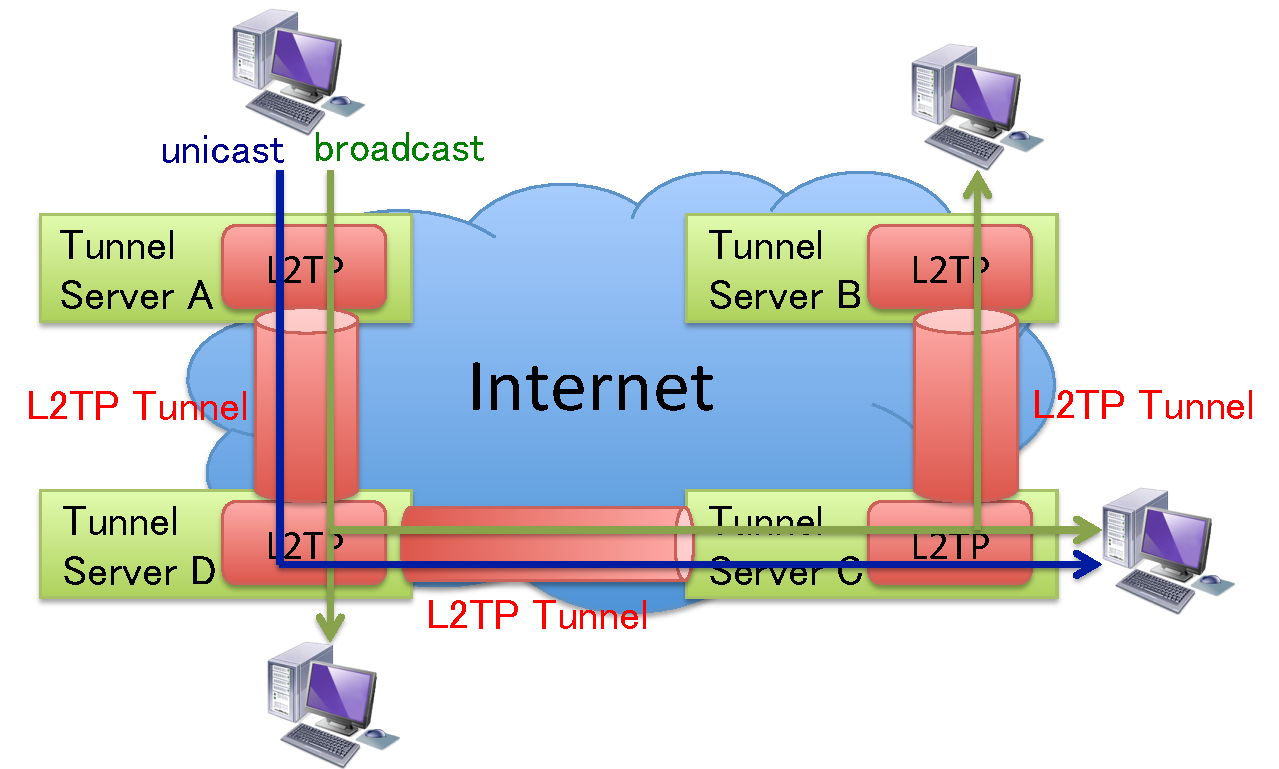
\includegraphics[scale=0.60]{./img/l2tptopology}
		\caption{L2TPを利用して拡張されたLayer 2ネットワーク}
		\label{img:l2tptopology}
	\end{center}
\end{figure}

一対一型のLayer 2ネットワーク技術は2つの拠点間で拡張されたLayer 2ネットワークを構築することができる。
一対一型のLayer 2ネットワーク拡張技術の例として、L2TP~\cite{rfc:l2tp}やGRE~\cite{rfc:gre}トンネルなどが挙げられる。L2TPを利用して
Layer 2ネットワークを拡張した際のトポロジーを図~\ref{img:l2tptopology}に示す。一対一型の
Layer 2ネットワーク拡張技術では2拠点間でLayer 2ネットワークを拡張する。3拠点以上
に同一のLayer 2ネットワークを拡張するためには、一対一型のLayer 2ネットワーク拡張技術を動作さえ、
全ての拠点に同一のLayer 2ネットワークを拡張する。そのため、図~\ref{img:l2tptopology}で示したような
トポロジーとなる。しかし、この手法では一部の拠点間で行われる通信の遅延が大きくなってしまうという問題がある。

Layer 2ネットワークのトポロジーは必ず木構造のトポロジーとなる。Layer 2スイッチはブロードキャスト
やマルチキャストのイーサネットフレームを受信すると、そのイーサネットフレームを受信したポート以外の全ポートにイーサネットフレーム
を転送する(=フラッディング)。フラッディングされたイーサネットフレームを受信したLayer 2スイッチは同様ににその
イーサネットフレームをフラッディングする。そのため、リング型のトポロジーでは、ブロードキャストストームや
マルチキャストストームが発生してしまうという問題(=L2ループ)が生じる。L2ループが生じると帯域がブロードキャストやマルチキャストの
イーサネットフレームで専有されてしまう上に、Layer 2スイッチのCPU負荷が高くなり正常にイーサネットフレームを
転送できなくなる。その結果、Layer 2スイッチに接続されているホスト同士も通信不能となってしまう。このような問題
を防ぐために、Layer 2ネットワークは木構造のトポロジーで構築される。また、Spanning Tree Protocol(=STP)を利用することで、
L2ループを発生させずにリング型のトポロジーを構築することも可能だが、
STPはL2ループを防ぐためにリングとなっているポートの通信を拒否する。その結果、STPを利用した場合でも、Layer 2ネットワークの
トポロジーは木構造のトポロジーとなってしまう。

\begin{figure}
	\begin{center}
		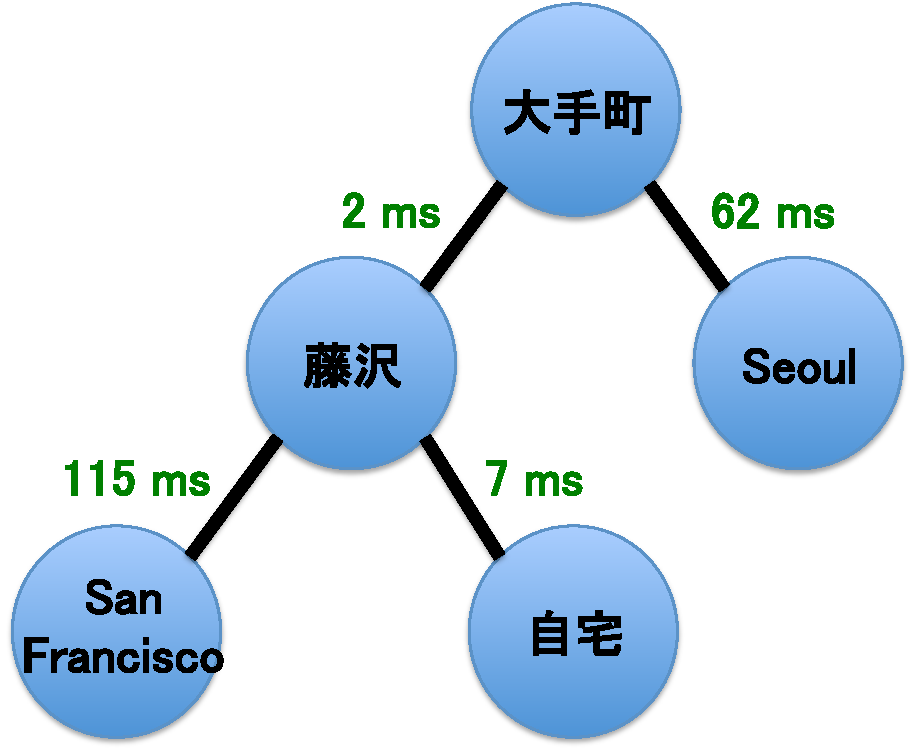
\includegraphics[scale=0.50]{./img/highlatencyl2}
		\caption{木構造となる広域Layer 2ネットワークのトポロジー例1}
		\label{img:highlatencyl2}
	\end{center}
\end{figure}

\begin{figure}
	\begin{center}
		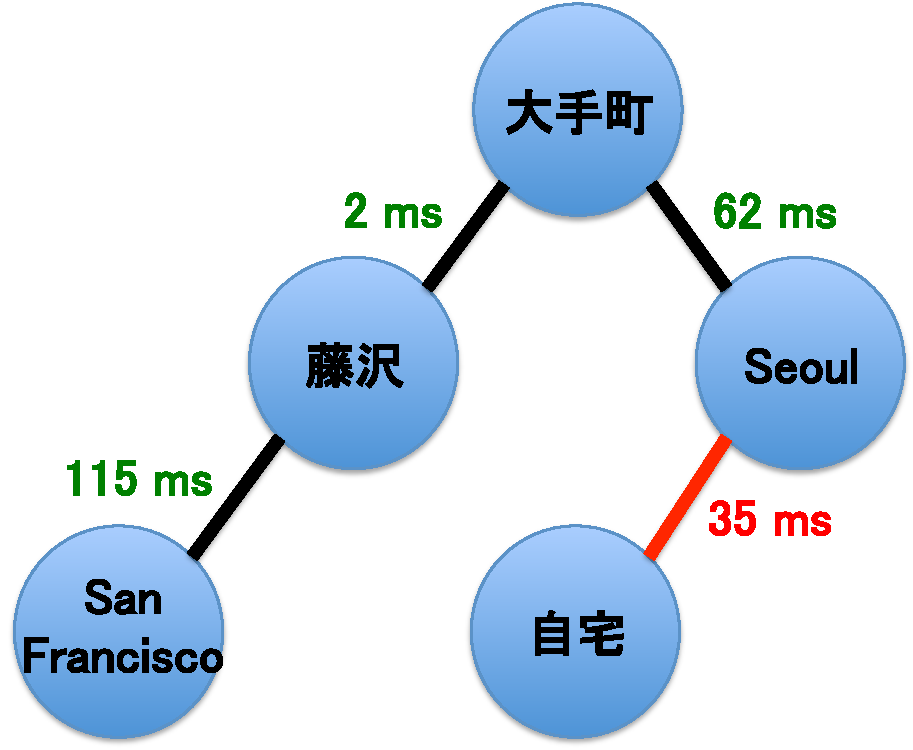
\includegraphics[scale=0.50]{./img/homeandseoul}
		\caption{木構造となる広域Layer 2ネットワークのトポロジー例2}
		\label{img:homeandseoul}
	\end{center}
\end{figure}

一対一型のLayer 2ネットワーク拡張技術を利用し、Layer 2ネットワークを複数の拠点に拡張した場合も
同様に木構造のトポロジーとなる。単一の拠点内で構築されるLayer 2ネットワークの場合、
Layer 2スイッチ間の遅延はほぼ無い状態なので、木構造のトポロジーでも問題とならない。しかし、Layer 2ネットワーク拡張技術を利用して
インターネット上に構築したLayer 2ネットワークでは、1ホップあたりの遅延が、単一の拠点内で構築したLayer 2ネットワークと比べ、非常に大きい。例えば、図~\ref{img:highlatencyl2}
で示すような広域なLayer 2ネットワークでは、自宅に設置されたホストとソウルに設置されたホスト間で通信を行った
場合、その遅延は71 msとなる。図~\ref{img:homeandseoul}で示すように、自宅とソウルを直接
接続した場合、遅延は35 msとなる。しかし、藤沢や大手町に設置されたホスト間で通信を行った
場合の遅延が97 ms以上となってしまう。このように、一対一型のLayer 2ネットワーク拡張技術では、
Layer 2ネットワークのトポロジーが木構造となってしまうため、必ず一部拠点間の遅延が大きくなってしまうという問題がある。


\section{一対多型のLayer 2ネットワーク拡張技術}
\label{rw:pointtomulti}

\begin{figure}
	\begin{center}
		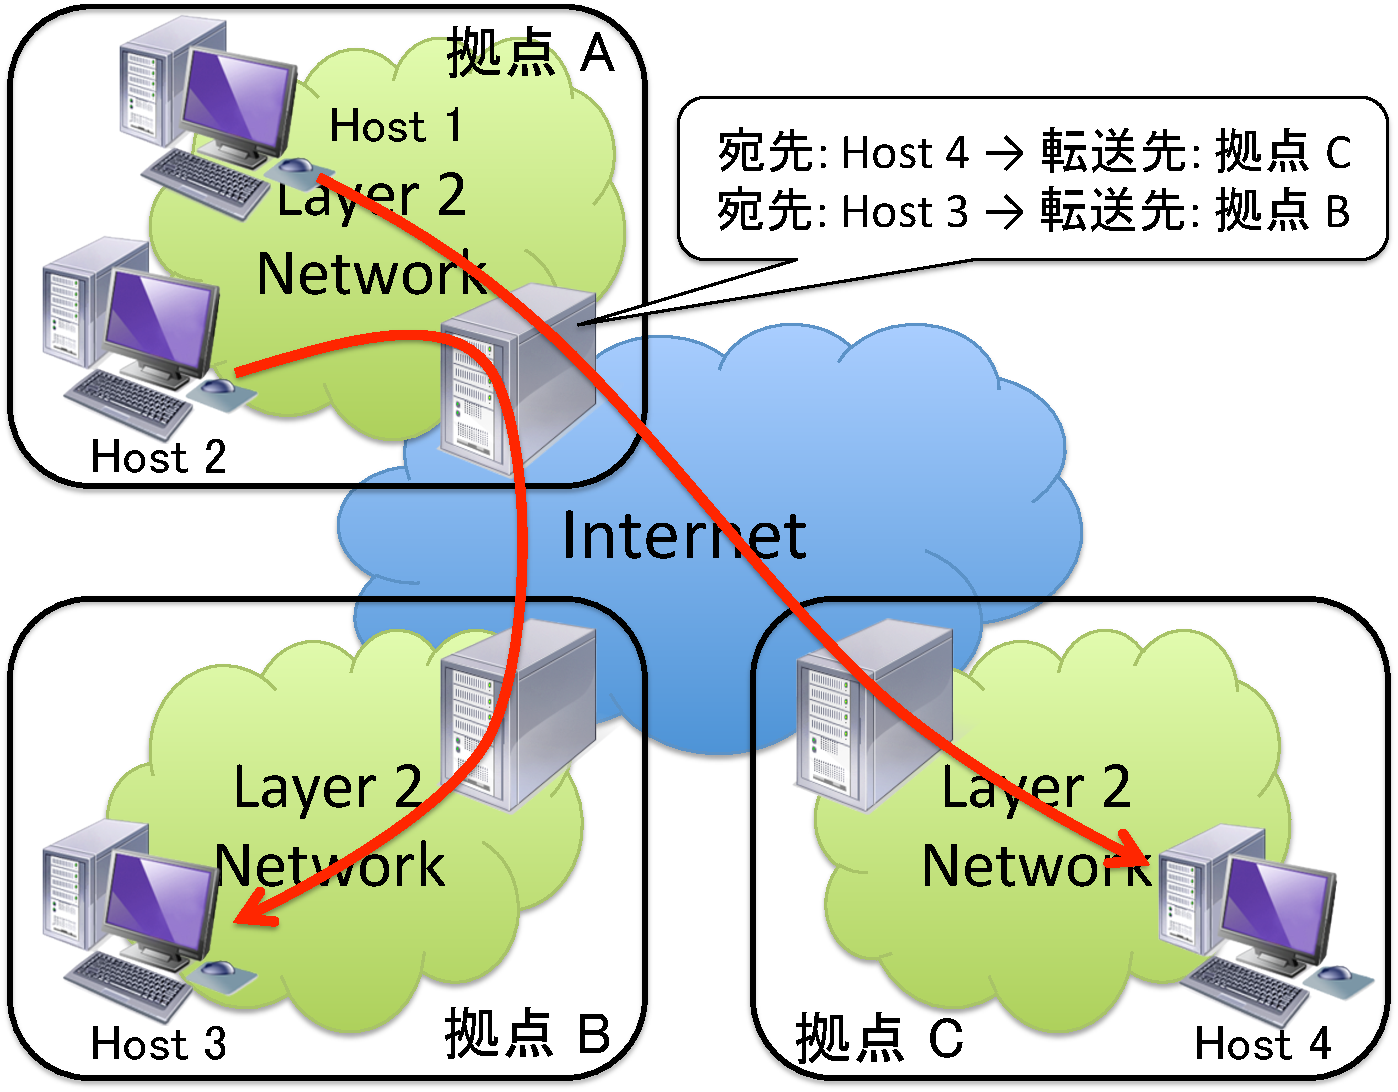
\includegraphics[scale=0.50]{./img/1tomulti}
		\caption{一対多型のLayer 2ネットワーク拡張技術}
		\label{img:1tomulti}
	\end{center}
\end{figure}

一対多型のLayer 2ネットワーク拡張技術は複数の拠点に対して同時にLayer 2ネットワークを拡張
することができる。一対一型のLayer 2ネットワーク拡張技術では、構築されたLayer 2ネットワーク
が木構造のトポロジーとなってしまうため、必ず一部拠点間の遅延が大きくなってしまうという問題がある。
この問題は、Layer 2ネットワーク拡張技術が、図~\ref{img:1tomulti}で示すように、
イーサネットフレームの宛先ホストに応じて転送するトンネル終端点の切り替えを行うことにより解決することが
できる。Layer 2ネットワーク拡張技術は、各拠点に設置されているホストを自動的に学習する。そして、
イーサネットフレームを転送する際には、宛先ホストがどのトンネル終端点によって収容されているか検索し、
そのトンネル終端点にイーサネットフレームを直接転送する。この手法では、一対一型のLayer 2ネットワーク拡張技術と比べると、
イーサネットフレームが宛先のトンネル終端点に直接
転送されるため、遅延の小さいLayer 2ネットワークを構築することができる。

一対多型のLayer 2ネットワーク拡張技術の例としてVirtual Extensible Local Area Network(=VXLAN)~\cite{id:vxlan}
とN2N~\cite{n2n}が挙げられる。これらの特徴を以下で述べる。

\subsection{VXLAN}
\label{rw:vxlan}

\begin{figure}
	\begin{center}
		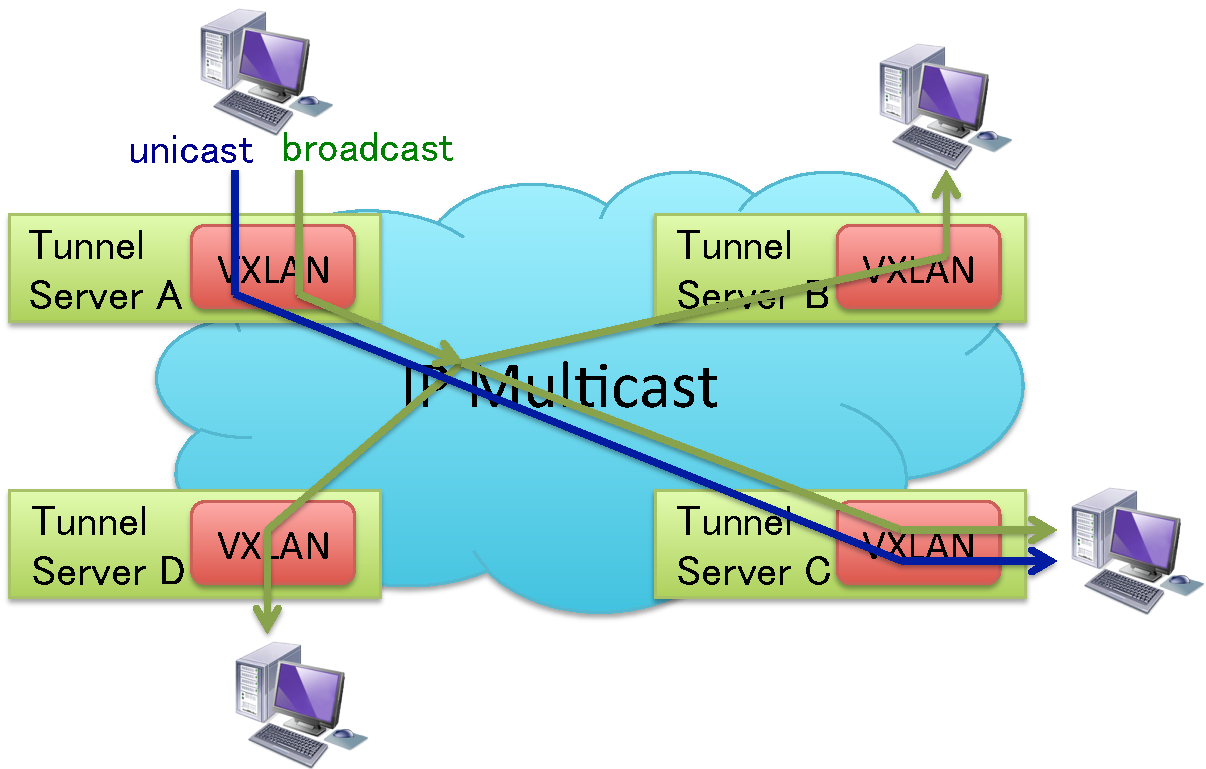
\includegraphics[scale=0.60]{./img/vxlantopology}
		\caption{VXLANを利用して拡張されたLayer 2ネットワーク}
		\label{img:vxlantopology}
	\end{center}
\end{figure}

VXLAN~\cite{id:vxlan}はCisco Systems社~\cite{cisco}やVMware社~\cite{vmware}を中心に提案されている一対多型のLayer 2ネットワーク拡張技術である。
VXLANを利用することにより、同一のLayer 2ネットワークを複数の拠点に拡張することができる。
VXLANを利用して複数の拠点に同一のLayer 2ネットワークを拡張した際のトポロジーとVXLANの
イーサネットフレーム転送手法を図~\ref{img:vxlantopology}に示す。
VXLANはトンネル終端点の検知やブロードキャストフレームの転送を行うために、IPマルチキャスト
を利用する。拡張されたLayer 2ネットワークに参加しているトンネル終端点は、全て同一の
IPマルチキャストグループに参加している。トンネル終端点が、収容しているホストからイーサネットフレームを
受信すると、まずそのイーサネットフレームの識別を行う。受信したイーサネットフレームが、ブロードキャストフレームの場合、
IPマルチキャストを利用してイーサネットフレームを転送する。全てのトンネル終端点は同一のIPマルチキャスト
グルームに参加しているため、IPマルチキャストグループに受信したイーサネットフレームを転送することにより、
イーサネットフレームは全てのトンネル終端点へ転送される。そして、他のトンネル終端点がそのイーサネットフレームを受信すると、
イーサネットフレームを収容しているホストへ転送する。また、イーサネットフレームを受信したトンネル終端点はイーサネットフレームの送信元ホストと
イーサネットフレームを転送したトンネル終端点を学習する。受信したイーサネットフレームがユニキャストフレームの場合、
まず、イーサネットフレームの宛先ホストが学習されているか確認する。学習されている場合、
受信されたイーサネットフレームを宛先ホストが収容されているトンネル終端点に直接転送する。学習されていない場合、
ブロードキャストフレームと同様に、IPマルチキャストを利用し全てのトンネル終端点へイーサネットフレームを転送する。
そして、宛先ホストが収容されているトンネル終端点がイーサネットフレームを受信すると、そのイーサネットフレーム
を宛先ホストへ転送する。VXLANは上記手法により、同時に複数の拠点に同一のLayer 2ネットワークを
拡張する。

VXLANを利用することにより、一対一型のLayer 2ネットワーク拡張技術で生じる木構造トポロジーの問題は解決
される。VXLANは転送されてきたイーサネットフレームの送信元ホストと転送したトンネル終端点を自動的に学習する。
そして、学習された情報を元に、転送すべきイーサネットフレームの宛先ホストに応じて転送先を自動的に選択する。
転送すべきイーサネットフレームがブロードキャストフレームの場合、または、学習されていないホスト宛のユニキャスト
フレームの場合はIPマルチキャストグループに転送する。学習されているホスト宛のユニキャストフレームの
場合は、宛先ホストが収容されているトンネル終端点に直接転送する。これにより、一対一型のLayer 2ネットワーク
拡張技術で生じる不要な中継がなくなるため、遅延は一対一型のLayer 2ネットワーク拡張技術と比べると小さくなる。

しかし、VXLANはインターネット上で動くように設計されていないため、VXLANを利用してインターネット上
に分散した複数の拠点に同一のLayer 2ネットワークを拡張するのは困難である。VXLANはトンネル終端点の
検知と一部イーサネットフレームの転送にIPマルチキャストを用いる。そのため、全てのトンネル終端点は同一の
IPマルチキャストグループに参加していることが求められる。しかし、インターネット上に分散した複数の
拠点に同一のIPマルチキャストグループを拡張することは困難である。XCast~\cite{rfc:xcast}やScatterCast~\cite{scattercast}などといった
IPマルチキャストを利用して、インターネット上に分散した複数の拠点に同一のIPマルチキャストグループを
拡張することは可能だが、Layer 2ネットワークを拡張をするために動かさなければいけないシステムが増える
ため、運用コストが高くなる上に障害発生時の問題切り分けも難しくなる。そのため、VXLANはインターネット上
の複数の拠点に同一のLayer 2ネットワークを拡張する手法として適切ではない。

また、VXLANを利用してインターネット上の複数の拠点に同一のLayer 2ネットワークを拡張した場合、
イーサネットフレームは遅延が最も小さい経路で転送されない。インターネット上の経路には~\ref{background:internetroute}節
で説明したように、直接転送した場合より、他のトンネル終端点を経由したほうが遅延が小さくなる場合がある。
VXLANはこのような経路が存在した場合でも、それを検知する仕組みが存在しないため、イーサネットフレームの転送は
必ず宛先のトンネル終端点に直接行う。そのため、拡張されたLayer 2ネットワークの遅延は最小限とならない。

\subsection{N2N}
\label{rw:n2n}

\begin{figure}
	\begin{center}
		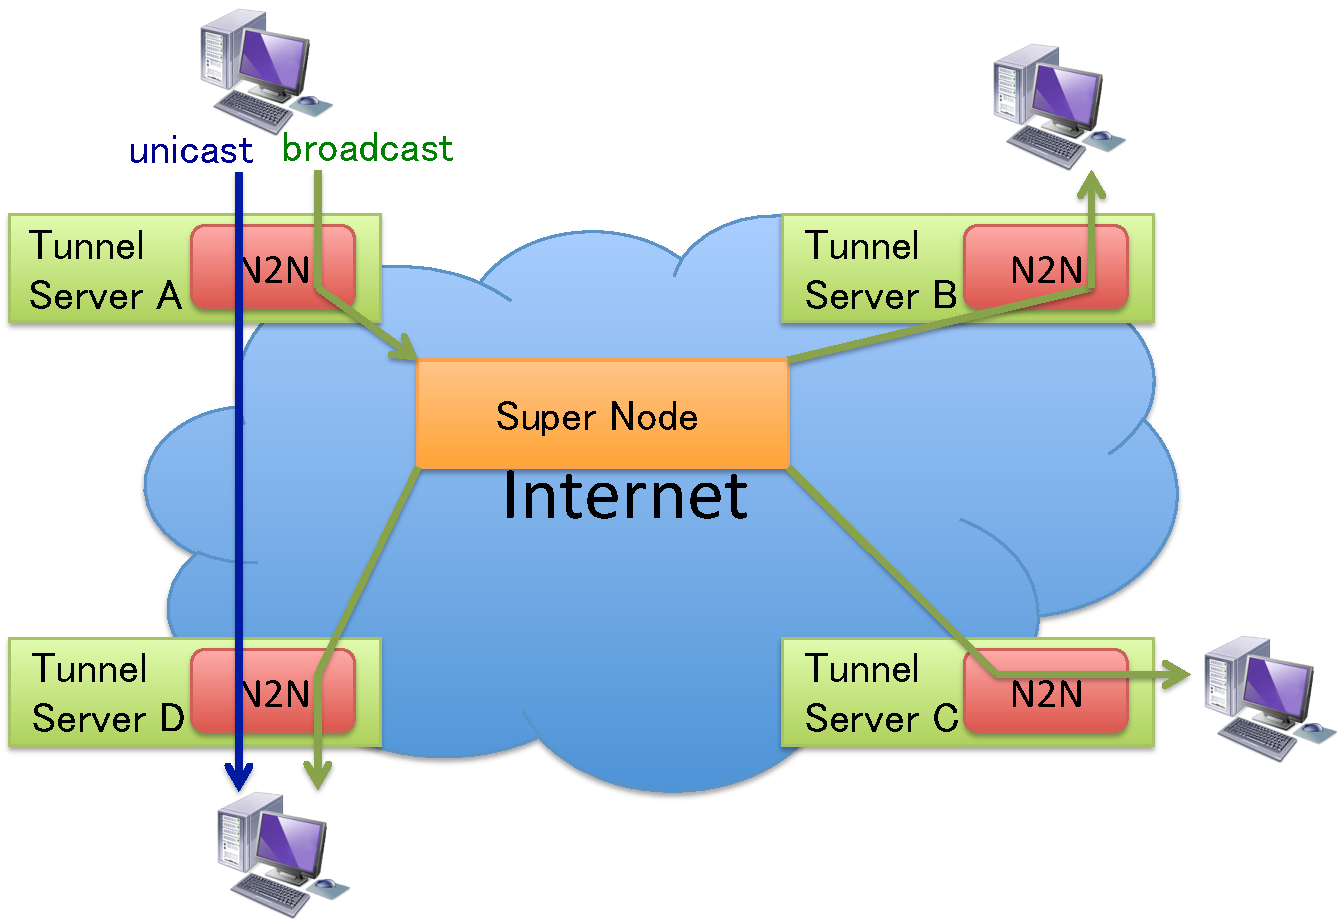
\includegraphics[scale=0.60]{./img/n2ntopology}
		\caption{N2Nを利用して拡張されたLayer 2ネットワーク}
		\label{img:n2ntopology}
	\end{center}
\end{figure}

N2N~\cite{n2n}はntop社~\cite{ntop}によって開発されている一対多型のLayer 2ネットワーク拡張技術である。
N2Nを利用することにより、インターネット上に分散した複数の拠点に同一のLayer 2
ネットワークを拡張することができる。N2Nを利用してインターネット上に分散した
複数の拠点に同一のLayer 2ネットワークを拡張した際のトポロジーとN2Nの
フレーム転送手法を図~\ref{img:n2ntopology}に示す。

N2Nはインターネット上に分散した複数の拠点に同一のLayer 2ネットワークを拡張する
ために、トンネル終端点とは別に、Supernodeというサーバーを用いる。Supernodeの役割
は大きく分けて2つある。1つ目の役割は、トンネル終端点の参加や離脱などといったコントロールメッセージ
の通知と管理である。Supernodeはトンネル終端点がLayer 2ネットワークへ参加した際に、Layer 2ネットワークに参加
している全トンネル終端点にそれを通知する。新規トンネル終端点はSupernodeのIPアドレスとポート番号を指定するだけで、Layer 2ネットワークに参加することができる。
2つ目の役割は、ブロードキャストフレームと一部ユニキャストフレームの転送である。
トンネル終端点がブロードキャストフレームを転送するためには、Supernodeにブロードキャストフレーム
を転送し、Layer 2ネットワークに参加している全トンネル終端点にブロードキャストフレームを転送してもらう。
これによりN2Nはインターネット上に分散した複数の拠点に同一のLayer 2ネットワークを
拡張することを可能としている。

N2Nはイーサネットフレームを宛先のトンネル終端点に直接転送するため、一対一型のLayer 2ネットワーク
拡張技術のように、一部通信の遅延が大きくなってしまうという問題が生じない。
N2Nによって拡張されたLayer 2ネットワークに参加しているホストがイーサネットフレームを
送信すると、N2Nのトンネル終端点はそのイーサネットフレームの転送を行う。トンネル終端点が
受信したイーサネットフレームがブロードキャストフレームの場合、トンネル終端点はそのイーサネットフレーム
をSupernodeに転送する。そして、Supernodeは受信したイーサネットフレームを全てのトンネル終端点
に転送する。Supernodeが再転送を行ったブロードキャストフレームをトンネル終端点が受け取ると、
収容しているホストにイーサネットフレームを転送した上で、送信元ホストと転送をしたトンネル終端点を学習する。
トンネル終端点が受信したイーサネットフレーム
がユニキャストフレームの場合、ユニキャストフレームの宛先ホストが学習されているホストかを確認する。
学習されているホストの場合は宛先ホストが収容されているトンネル終端点にイーサネットフレームを直接
転送する。学習されていないホストの場合はブロードキャストフレームと同様に、Supernodeへ転送し、全
トンネル終端点に転送を行なってもらう。N2Nはこのようにイーサネットフレームを宛先のトンネル終端点
に直接転送をするため、遅延は一対一型のLayer 2ネットワーク拡張技術と比べ小さくなる。

しかし、N2Nは~\ref{background:internetroute}節で説明したようなインターネットの経路が考慮されていない。
また、一部のイーサネットフレームは必ずSupernodeを経由する。そのため、遅延が最も小さい経路で転送されていないと言える。N2Nにはトンネル終端点間の
遅延を計測し、その計測結果に基いて遅延が最も小さい経路を選択する仕組みが存在しない。そのため、
他のトンネル終端点を経由することにより遅延が小さくなるような経路が存在したとしても、イーサネットフレーム
は宛先のトンネル終端点に直接転送される。また、ブロードキャストフレームや一部のユニキャストフレームは必ず
Supernodeを経由する。そのため、トンネル終端点からSupernodeまでの遅延が大きい場合や、Supernodeの負荷が高い
場合は遅延が大きくなってしまう。よって、N2Nではインターネット上に分散した複数の拠点に拡張されたLayer 2ネットワーク
の遅延は最小限とならない。

更にN2NはSupernodeが単一障害点となっている。N2Nは一部イーサネットフレームの転送にSupernodeを用いている。
また、Layer 2ネットワークに参加しているトンネル終端点の管理はSupernodeが行なっている。そのため、
Supernodeで障害が発生した場合、拡張されたLayer 2ネットワークが完全に利用できなくなってしまうという問題がある。

\section{関連研究の比較}
\label{background:korekara}

本節では、~\ref{rw:pointtopoint}節、~\ref{rw:pointtomulti}節で説明したLayer 2ネットワーク拡張技術について、
インターネット上に分散された複数の拠点に同一のLayer 2ネットワークを拡張した際に、拡張されたLayer 2ネットワーク上で
動作するサービスの遅延によるパフォーマンス低下を小さくするという目的に向けた観点から比較、検討を行う。これを実現するための
要件は以下の通りである。

\begin{itemize}
	\item{宛先に応じた転送先の選択が可能である}
	\item{遅延が最も小さくなる経路の選択が可能である}
	\item{インターネット上で動作する}
	\item{分散して動作する}
\end{itemize}

目的を実現するための各要件について、~\ref{rw:pointtopoint}節と~\ref{rw:pointtomulti}節で挙げた既存研究が
どの程度満たしているかを表~\ref{table:relatedworks}に示す。

\begin{table}[h]
	\begin{center}
		\caption{既存研究の比較}
		\begin{tabular}{|c|c|c|c|c|}
			\hline
			既存研究 & 転送先の選択 & 遅延に基づいた経路選択 & インターネットでの動作 & 分散 \\
			\hline
			\hline
			L2TP,GRE & × & × & ◯ & × \\
			VXLAN & ◯ & × & × & ◯ \\
			N2N & ◯ & × & ◯ & × \\
			\hline
		\end{tabular}
		\label{table:relatedworks}
	\end{center}
\end{table}

~\ref{background:thisresearch}節で説明したように、インターネット上に分散された複数の拠点に拡張した
Layer 2ネットワークで動作するサービスの遅延によるパフォーマンス低下を小さくするためには、イーサネット
フレームを遅延が最も小さくなる経路で転送する。L2TPやGREといった一対一型のLayer 2ネットワーク拡張技術
は、転送先をイーサネットフレームの宛先に応じて選択することができない。そのため、Layer 2ネットワークの
トポロジーは木構造となるため、一部通信の遅延は大きくなる。一方、N2NとVXLANは宛先に応じて転送先を選択
することができる。しかし、N2NとVXLANには、トンネル終端点間の遅延を計測し、その計測結果に基いて遅延が
最も小さくなる経路を選択する仕組みがない。そのため、転送する際の経路が、必ずしも遅延の最も小さい経路
ではないという問題がある。

また、インターネット上に分散された複数の拠点に同一のLayer 2ネットワークを拡張するためには、Layer 2ネットワーク
拡張技術がインターネット上で動作する必要がある。L2TP、GREとN2Nはインターネット上で動作するように設計されている。
しかし、VXLANは他トンネル終端点の検知と一部イーサネットフレームの転送にIPマルチキャストを用いているため、
インターネット上では動作しないという問題がある。

更に、~\ref{background:ml2}項で説明したように、1つの拠点で発生した障害によるサービスの停止を防ぐために、
複数の拠点を利用する場合が多い。拡張されたLayer 2ネットワークが、ある拠点で発生した障害の影響を受け、
利用できなくなっては複数拠点の利点を得ることが出来ない。VXLANは分散して動作しているため、IPマルチキャストが
正常に動作していれば、障害の影響は受けない。一方で、L2TPとGREは木構造のトポロジーとなるため、ある拠点で
障害が発生すると拡張されたLayer 2ネットワークでも障害が発生する、という問題がある。また、N2NはSupernodeを利用してSupernodeの
管理と一部イーサネットフレームの転送を行なっているため、Supernodeが設置されている拠点で障害が発生すると、
Layer 2ネットワークで一切通信ができなくなる、という問題がある。

%\begin{figure}
%	\begin{center}
%		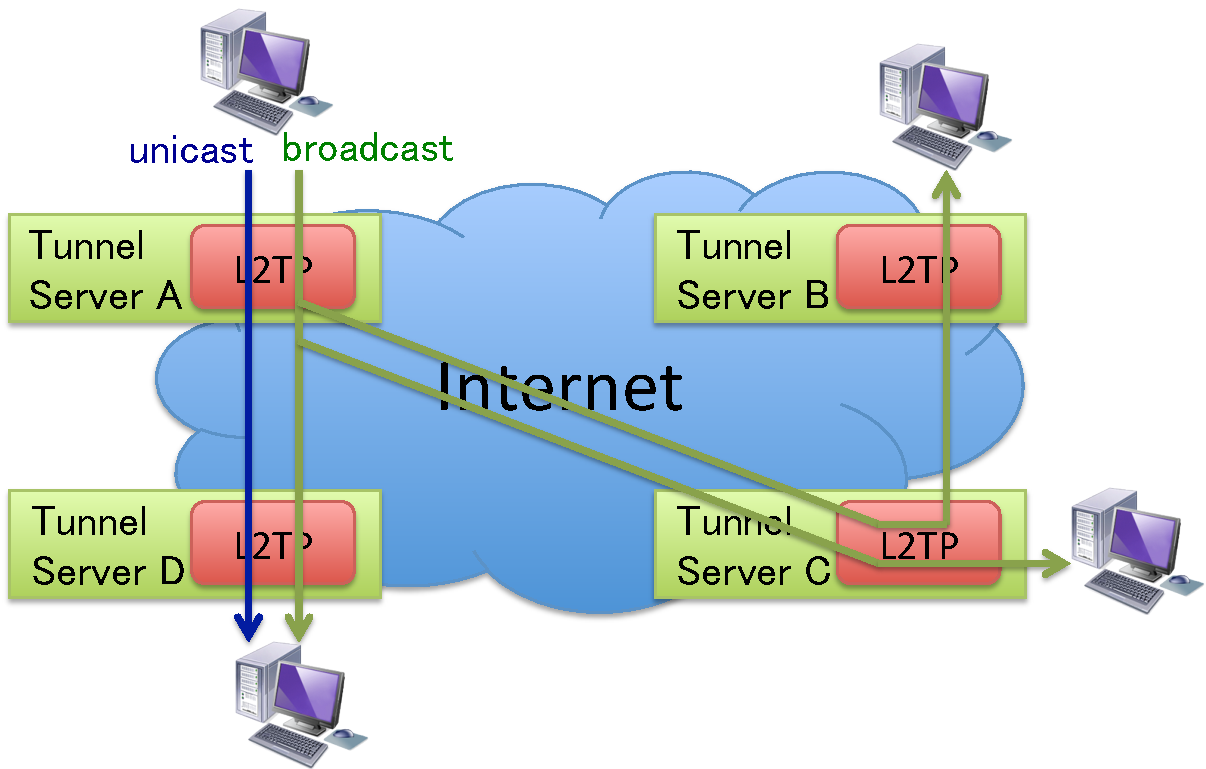
\includegraphics[scale=0.60]{./img/leontopology}
%		\caption{求められるLayer 2ネットワーク拡張技術}
%		\label{img:reqtopology}
%	\end{center}
%\end{figure}

%%% Local Variables:
%%% mode: japanese-latex
%%% TeX-master: "../yummy_bthesis"
%%% End:
